\chapter{Ergebnisse und Diskussion}

Im Fokus dieses Kapitels stehen die Ergebnisse und Diskussionen im Kontext der Evaluierung von Dichteeigenschaften und Schrumpfungsverhalten des 316L-Edelstahls von \textit{PT+A} für den 3D-Druck mittels Fused Deposition Modeling (FDM). Im vorangegangenem Kapitel wird die Erstellung der Proben und die Wissenschaftlichen Grundlagen erläutert.

\section{Dichte- und Schwindungsauswertungen der gedruckten Proben}

In diesem Unterkapitel werden die gedruckten Würfel- und Zugproben hinsichtlich der Dichte untersucht. Diese Messung wird einmal im Grün-, sowie im Braun-, als auch im späteren Sinterteil durchgeführt. Die Ergebnisse dieser Auswertung ist in \autoref{Grünteilmaße} bis \autoref{Sinterteilmaße} dargestellt.
Aus diesen Werten lassen sich die Schwindungen der einzelnen Parameter nach jedem Prozess ableiten. Dargestellt sind diese Werte in \autoref{Schrumpfung}.

\begin{table}[h]
    \centering
    \caption{Schrumpfung der Würfelproben im Braun- und Sinterteil}
      \begin{tabular}{ccccccc}
      \toprule
      \textbf{Teil} & \multicolumn{1}{c}{\textbf{h}} & \multicolumn{1}{c}{\textbf{l1}} & \multicolumn{1}{c}{\textbf{l2}} & \multicolumn{1}{c}{\textbf{V}} & \multicolumn{1}{c}{\textbf{m}} & \multicolumn{1}{c}{\textbf{Dichte}} \\
        \textbf{Braunteil} & 0 & 2,9 & 2,9 & 5,8 & 4,8 & -0,8 \\
        \textbf{Sinterteil} & 13,7 & 15,4 & 15,8 & 38,6 & 8 & -50 \\
      \bottomrule
      \end{tabular}%
    \label{Schrumpfung}%
  \end{table}%
  \FloatBarrier

Auffällig ist die völlige Schrumpfung des Volumens, welche erst nach dem Sinterprozess anliegt. Die Massenschwindung nach beiden Prozessen lässt sich mit der Verflüchtigung von dem Bindermaterial erklären. 
Von den liegenden Zugproben wurden auch Masse und Gewicht gemessen. Daher lassen sich auch hier das Schrumpfungsverhalten darstellen. Diese Werte sind in \autoref{Schrumpfung Zugproben} angegeben.


\begin{table}[h]
    \centering
    \caption{Schrumpfung der liegenden Zugproben im Sinterteil}
      \begin{tabular}{ccccccc}
      \toprule
      \textbf{Teil} & \multicolumn{1}{c}{\textbf{l1}} & \multicolumn{1}{c}{\textbf{l2}} & \multicolumn{1}{c}{\textbf{V}} & \multicolumn{1}{c}{\textbf{m}} & \multicolumn{1}{c}{\textbf{Dichte}} \\
        \textbf{Sinterteil} & 13,7 & 15,4 & 15,8 & 38,6 & 8 & -50 \\
      \bottomrule
      \end{tabular}%
    \label{Schrumpfung Zugproben}%
  \end{table}%
  \FloatBarrier

\section{Ergebnisse der Zugversuche}

In diesem Abschnitt werden die mechanischen Kennwerte des 316L-Edelstahls mittels eines Zugversuchs ermittelt. Dazu wird mithilfe des, in \autoref{Drucker} vorgestellten, FDM-Drucker Zugproben hergestellt. Diese Zugproben sind nach DIN 50125-E3x8x30 hergestellt.
Geplant war es, die Zugproben liegend und stehend auf der Druckoberfläche zu drucken und zu sintern. Jedoch bildeten die stehenden Zugproben (in \autoref{stehende Zugprobe} dargestellt) Probleme.

\begin{figure}[h] 
  \centering
  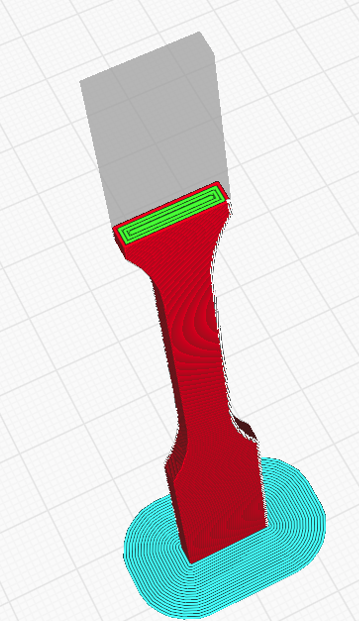
\includegraphics[width=0.5\linewidth]{bilder/Screenshot 2023-11-01 171423.png}
        \caption[Stehende Zugprobe im Cura-Slicer] {Stehende Zugprobe im Cura-Slicer (Quelle: \autocite{Prusa})}
  \label{stehende Zugprobe}
\end{figure}
\FloatBarrier

Da die Querschnittsfläche einer stehenden Zugprobe deutlich kleiner ist, als bei den liegenden Zugproben, führte dies zu Problemen. Daher wird sich im Rahmen dieser Arbeit auf den Vergleich zwischen den liegenden Zugproben hinsichtlich der mechanischen Kennwerte bezogen.
Im Slicer sind dann in x- und y-Richtung um 17\% vergrößert und in z-Richtung sind sie 20\% größer gedruckt. Damit ist sichergestellt, dass die Zugproben im gesinterten Zustand die DIN-Norm einhalten. Die fertig gesinterten Zugproben werden dann in eine Zugprüfmaschine an beide Seiten eingespannt und bis zur Zerstörung gezogen. Die benötigte Kraft, sowie die entstehende Längung bilden die Grundlage für das entstehende Spannungs-Dehnungs-Diagramm.
Das zugehörige Spannungs-Dehnungs-Diagramm ist in \autoref{label}

\section{Vergleich der ermittelten Werte}

